%!TEX root = ../thesis.tex
%Adding the above line, with the name of your base .tex file (in this case "thesis.tex") will allow you to compile the whole thesis even when working inside one of the chapter tex files

\chapter{Multi-wavelength Radio Continuum Emission Studies of \\ Dust-free Red Giants} \label{chap:6}

\section{Introduction}\label{sec:6.1}
\section{$\alpha$ Boo Radio Maps}\label{sec:6.2}
\section{$\alpha$ Tau Radio Maps}\label{sec:6.3}
\section{Results vs Previous Observations}\label{sec:6.4}
Prior to and during the early operation of the `old' VLA, a small number of single dish radio observations reported the detection of flares from single red giants (e.g., \citealt{slee_1989}). These transient radio events have never been re-observed however, even with more sensitive interferometers, suggesting that such detections were spurious (e.g., \citealt{beasley_1992}). The first definitive detection of thermal free-free emission from a luminosity class III single red giant at centimeter wavelengths was of $\alpha$ Boo at 6 cm \citep{drake_1983,drake_1986}. Since then there has been a modest number of centimeter and millimeter observations of this star. In Table \ref{tab:6.4.1} we list the majority of these observations and plot their flux densities as a function of frequency in Figure x. In comparison to other single red giants, $\alpha$ Boo had been relatively well observed at radio continuum wavelengths before this study, including detections in four VLA bands (i.e., Q, K, Ku, and C). No Ku band receivers were available during the commissioning phase of the VLA in early 2011 so we can compare three of our detections with previous ones. \\

\begin{table}[!hb]
\begin{center}
\caption[Compilation of Previous Radio Observations ($\nu \le 250$ GHz).]
{Compilation of Previous Radio Observations ($\nu \le 250$ GHz).}
\begin{tabular}{cccccc}
\hline
\hline
\rule{0pt}{2.5ex}Source & $\nu$ (GHz) & Date &  $F_{\nu}$ (mJy) & S/N & Reference\\
\hline
$\alpha$ Boo &4.9  & 1983 Jan 21 & 0.39 & 3.0 & 1 \\
&4.9  & 1983 May 20 & 0.26 & 3.3& 1 \\
&4.9  & 1983 Dec 26 & $\le$0.18$(3\sigma)$&- & 1 \\
&4.9  & 1984 Mar 17 & 0.24  & 4.8& 1 \\
&15.0 & 1984 Nov 6 & 0.68 & 7.6& 1 \\
&22.5  & 1999 Jan 06  &1.7& 8.5& 2 \\
&43.3  & 1999 Jan 06 & 3.3& 8.3& 2 \\
&43.3  & 2004 Jan 25 & 3.34& 41.8& 2 \\
&86.0  & 1985 Nov  & 21.4& 3.0& 3 \\
&108.4  & 1997 Nov - 2000 Jun & 20.1 &29.1 & 4 \\
&217.8 & 1997 Nov - 2000 Jun  & 83.5 &48.8 & 4 \\
&250.0  & 1986 Dec - 1989 Mar  & 78.0 & 9.8& 5 \\
\hline
\rule{0pt}{3ex}    $\alpha$ Tau	&4.9  & 1983 Jan 21 & $\le$0.27$(3\sigma)$&-& 1 \\
&4.9  & 1984 Nov 6 & $\le$0.22$(3\sigma)$&-& 1 \\
&5.0  & 1997 Sep 27 & $\le$0.07$(3\sigma)$	&-& 6 \\
&8.5  & 1997 Sep 27 & 0.28 	&9.3	& 6 \\
&14.9 & 1997 Sep 27 & 0.95 	&11.9	& 6 \\
&15.0 & 1984 Nov 6 & 0.60 	&6.0	& 1 \\
&108.4  & 1997 Nov - 2000 Dec &  14.0  & 9.6& 4 \\
&217.8 & 1999 Sep - 2000 Dec  & 25.8 & 4.6& 4 \\
&250.0  & 1986 Dec - 1987 Jan & 51.0 & 8.5& 5 \\
\hline
\end{tabular}
\label{tab:6.4.1}
\begin{minipage}{13.5cm}
\rule{0pt}{3ex} References.-(1)\cite{drake_1986}; (2)\cite{dehaes_2011}; (3)\cite{altenhoff_1986}; (4) \cite{cohen_2005}; (5) \cite{altenhoff_1994}; (6) \cite{wood_2007}; 
\end{minipage}
\end{center}
\end{table}

Previous detections of $\alpha$ Boo at 6 cm ranged from a 3$\sigma$ upper limit of 0.18 mJy to a 3$\sigma$ detection at 0.39 mJy. Our 6 cm value agrees to within $\sim$10$\%$ of the highest S/N (5$\sigma$) value of \cite{drake_1986}. There is no significant difference between our 1.3 cm value and that of \cite{dehaes_2011}. There is however a notable difference in flux density values at 0.7 cm  where \cite{dehaes_2011} report values that are lower than ours by over 40\%. Such a level of chromospheric variability seems rather high and would be unexpected from such supposedly inactive stars \citep{harper_2013}. Another possibility for the difference in values is that the longer cycle time used by \cite{dehaes_2011}, which was over double our value, may lead to larger phase errors and thus lower final flux density values. Future high frequency VLA observations of $\alpha$ Boo will clarify this discrepancy at 0.7 cm but past detections at longer wavelengths appear to be in good agreement with our data.

In Figure x we plot the previous  radio measurements of $\alpha$ Tau at all frequencies below 250 GHz (i.e. 0.12 cm). Prior to this study, $\alpha$ Tau had only been detected at two VLA bands (i.e., X and Ku) and had never been detected at wavelengths longer than 3 cm due to its relatively low mass-loss rate. Our lack of a Ku-band measurement means that we can only compare the previous 3 cm detection reported in \cite{wood_2007} to ours. We find that there is no significant difference between the two. Interestingly, \cite{wood_2007} report a non-detection of $\alpha$ Tau at 6 cm and placed a 3$\sigma$ upper limit of 0.07 mJy on its emission. In stark contrast to this, we were able to detect the star at 6 cm with a flux density over two times greater than this value. This hint of variability at long wavelengths would be consistent with the predictions of the broadband nonlinear Alfv\'{e}n wave model of \cite{airapetian_2010} but can only be confirmed with future high S/N observations.
\section{Results vs Existing Models}\label{sec:6.5}
\section{Constraining $\alpha$ Tau's Molsphere}\label{sec:6.5a}
\section{Estimation of Mass Loss Rates from the \\ Radio Data}\label{sec:6.5b}
\section{Spectral Indices}\label{sec:6.6}
Long wavelength radio emission from non-dusty K spectral-type red giants is due to thermal free-free emission in their partially ionized outflows while shorter wavelength radio emission emanates from the near static and more ionized lower atmospheric layers. The radio flux density-frequency relationship for these stars is usually found to be intermediate between that expected from the isothermal stellar disk emission, where $\alpha$ follows the Rayleigh-Jeans tail of the Planck function (i.e., $\alpha = +2$), and that from an optically thin plasma (i.e., $\alpha = -0.1$). We have shown in Chapter 1 that the expected radio spectrum from a spherically symmetric isothermal outflow with a constant velocity and ionization fraction varies as $\nu ^{0.6}$ \citep{wright_1975,olnon_1975,panagia_1975}. In reality however, thermal gradients will exist in the outflow when the heating mechanisms become insufficient to counteract adiabatic and line cooling, so one would expect a temperature decrease in the wind at some point. Also, if the radio emission emanates from the wind acceleration zone then the electron density will not follow $n_{e} \propto r^{-2}$. 

We therefore relax some of the constant property wind model assumptions and assume that the electron density and temperature vary as a function of distance from the star $r$, and have the power-law form $n_{e} \propto r^{-p}$ and $T_{e} \propto r^{-n}$, respectively \citep[e.g.,][]{seaquist_1987}. Finding the spectral index for an outflow with these conditions is non-trivial so we highlight the main steps required to do so here. We assume the same geometry and notation used for the constant property wind model in Chapter 1, and again start by calculating the total optical depth for a ray with an impact parameter $b$, through the atmosphere:
\begin{equation}
\tau_{\nu} =\frac{0.212Z^2n^2_{\rm{e}}(R_{0})R_{0}^{2p}}{T^{1.35}\nu^{2.1}T_{e}^{1.35}(R_{0})R_{0}^{1.35n}}\int ^{\infty}_{-\infty} \frac{1}{(b^2 + z^2)^{(1.35n -2p)/2}} dz.
\label{eq:eq6.6.1}
\end{equation}
This integral can be solved using the relationship
\begin{equation}
\int ^{\infty}_{-\infty} \frac{1}{(b^2+z^2)^{t/2}} dz = b^{1-t}\sqrt{\pi}\left[\frac{\Gamma(t/2-0.5)}{\Gamma (t/2)} \right]
\label{eq:eq6.6.2}
\end{equation}
and setting $t=(1.35n -2p)$. Here $\Gamma$ is the gamma function i.e., $\Gamma (y)= \int ^{\infty}_{0} u^{y-1}e^{-u}du$. The total optical depth along a ray is then 
\begin{equation}
\tau_{\nu}(b) = Gb^{1-2p +1.35n}
\label{eq:eq6.6.3}
\end{equation}
where $G$ is a constant that incorporates $\nu$. As the total flux density is
\begin{equation}
F_{\nu} = \frac{2\pi}{D^2}\int ^{\infty}_{0} B_{\nu}[1 - e^{-\tau_{\nu}(b)}]bdb,
\label{eq:eq6.6.4}
\end{equation}
we can now substitute in the Rayleigh Jeans function for $B_{\nu}$ (remembering that $T_{e}$ now depends on distance from the star) to get
\begin{equation}
F_{\nu}=\frac{4\pi k\nu^2 T_{e}(R_{0})R_{0}^{n}}{D^2c^2}\int ^{\infty}_{0}(1-e^{-\tau _{\nu}})(b^2+z^2)^{-\frac{n}{2}}bdb.
\label{eq:eq6.6.5}
\end{equation}
Expansion of the second term inside the integral gives
\begin{equation}
F_{\nu} \simeq \frac{4\pi k\nu^2 T_{e}(R_{0})R_{0}^{n}}{D^2c^2}\int ^{\infty}_{0}(1-e^{-\tau _{\nu}})b^{1-n}db
\label{eq:eq6.6.6}
\end{equation}
To progress further, Equation \ref{eq:eq6.6.3} can be rearranged to find $b$ and $db$ in terms of $\tau _{\nu}$, and can then be inserted into Equation \ref{eq:eq6.6.6} to give
\begin{equation}
F_{\nu} \simeq \frac{4\pi k\nu^2T_{0}(R_{0})R_{0}^{n}}{D^2c^2}\int ^{\infty}_{0}(1-e^{-\tau _{\nu}})\left(\frac{\tau _{\nu}}{G} \right)^{\frac{1-2.35n +2p}{1-2p +1.35n}}\frac{d\tau _{\nu}}{G(1-2p + 1.35n)}.
\label{eq:eq6.6.7}
\end{equation}
This allows $\nu$ to be separated out to give
\begin{equation}
F_{\nu} \propto \nu^2 G^{\frac{2.35n -2p -1}{1-2p +1.35n}} G^{-1}
\label{eq:eq6.6.8}
\end{equation}
and as $G \propto \nu^{-2.1}$ we get
\begin{equation}
F_{\nu} \propto \nu^2 \nu^{\frac{4.2-2.1n}{1-2p +1.35n}},
\label{eq:eq6.6.9}
\end{equation}
i.e.,
\begin{equation}
\alpha = \frac{4p -6.2 -0.6n}{2p-1-1.35n}.
\label{eq:eq6.6.10}
\end{equation}
Therefore, if the spectral index of a stellar outflow can be measured, and if we make an assumption about the property of either the thermal or electron density profile of the wind, then Equation \ref{eq:eq6.6.10} provides us with information on how the other value varies.

\begin{figure}[hbt!]
\centering 
          \includegraphics[trim=0pt 0pt 10pt 30pt,clip,width=11.0cm, angle=90]{/home/eamon/thesis/thesis_template/6/spec_index.ps}
\caption[Power law fits to the spectra of $\alpha$ Boo and $\alpha$ Tau.]{Radio spectra for $\alpha$ Boo and $\alpha$ Tau, together with the best fit power law to their long wavelength flux densities and the resulting spectral indices. The spectral indices for $\alpha$ Boo and $\alpha$ Tau are found to be 1.05 and 1.58, respectively, which are both larger than the 0.6 value expected for a constant property wind model.}
\label{fig6.6.1}
\end{figure}

The radio spectra for both stars are shown in Figure \ref{fig6.6.1}, together with the power laws that were fitted to the long wavelength flux densities by minimizing the chi-square error statistic. For $\alpha$ Boo, a power law with $F_{\nu} \propto \nu ^{1.05 \pm 0.05}$ fits the four longest wavelength data points well. This spectral index is larger than the 0.8 value obtained by \cite{drake_1986} whose value was based on a shorter wavelength (2 cm) value and a mean value of four low S/N measurements at 6 cm. $\alpha$ Tau was found to have a larger spectral index and a power law with $S_{\nu} \propto \nu ^{1.58 \pm 0.25}$ best fitted the three longest wavelength data points. This value is in agreement with \cite{drake_1986} who report a value $\ge 0.84$ and is lower than the value of 2.18 that can be derived from the shorter wavelength data given in \cite{wood_2007}. It should be emphasized that the spectral index for both stars is a lot steeper than that expected from the constant property wind model. 

\begin{figure}[hbt!]
\centering 
          \includegraphics[trim=0pt 30pt 10pt 60pt,clip,width=11.0cm, angle=90]{/home/eamon/thesis/thesis_template/6/den_temp_coef.ps}
\caption[Variation of density and temperature coefficients for $\alpha$ Boo and $\alpha$ Tau.]{The variation of density and temperature coefficients for the empirically derived spectral indices. The density coefficients for an isothermal flow ($n$=0) along with the temperature coefficients for a constant outflow velocity ($p$=2) are also shown for both stars.}
\label{fig6.6.2}
\end{figure}

Equation \ref{eq:eq6.6.10} can be used in conjunction with our new spectral index for each star to calculate the density and temperature coefficients that may describe their outflows. The combinations of the electron temperature and density coefficients are shown for each star in Figure \ref{fig6.6.2} along with the coefficients obtained by assuming either an isothermal flow or a constant velocity flow. One explanation for spectral indices of stellar outflows being larger than 0.6 is that the wind is still accelerating in the radio emitting region, if the thermal gradients are assumed to be small. Ignoring thermal gradients may be reasonable over the wind acceleration region since it is probable that some form of Alfv\'en waves are required to lift the material out of the gravitational potential. These waves would need to have large damping lengths and undergo some dissipation within a few stellar radii of the surface in order to produce the low terminal velocities \citep{hartmann_1980}. These large damping lengths could result in shallow thermal gradients close in. If we ignore thermal gradients, then the density coefficients are $p=$2.71 and 5.5 for $\alpha$ Boo  and $\alpha$ Tau, respectively. This assumption is reasonable at short wavelengths where the majority of the radio emission is expected to emanate from the chromosphere or wind acceleration zone, but at long VLA wavelengths (i.e., between 6 and 20 cm) we may indeed be sampling the wind very close to or at its terminal velocity and the wind may have substantial thermal gradients caused by adiabatic cooling. 

To investigate this matter further,  we estimate the effective radius of the radio emitting region as a function of wavelength based on the Drake model for $\alpha$ Boo and the hybrid McMurry and Robinson model for $\alpha$ Tau. We follow the approach used by \cite{cassinelli_1977} and assume that the radio emission at each wavelength emanates from a surface at radial optical depth $\tau _{\rm{rad}}=$1/3. This is a modification of the Eddington-Barbier relation for an extended atmosphere where emission from smaller optical depths has added weight. Since the radio free-free opacity increases at longer wavelengths the optical depth along a line of sight into the stellar outflow also increases at longer wavelengths. This implies that the effective radius (i.e., the radius where $\tau _{\lambda} = \tau _{\rm{rad}}$) will increase with longer wavelengths and will be greater for outflows with higher densities of ionized material as $\tau _{\lambda} \propto \lambda ^{2.1}\int n_{\rm{ion}}(r)n_{\rm{e}}(r) dr$. 

\begin{figure}[hbt!]
\centering 
          \includegraphics[trim=0pt 20pt 10pt 40pt,clip,width=11.0cm, angle=90]{/home/eamon/thesis/thesis_template/6/eff_rad.ps}
\caption[Predicted effective radius as a function of wavelength for $\alpha$ Boo and $\alpha$ Tau.]{Predicted effective radius (dashed lines) as a function of wavelength derived from the existing atmospheric models of $\alpha$ Boo and $\alpha$ Tau.  Also plotted is the predicted effective radius derived from our analytical advection model for $\alpha$ Boo (discussed in Section \ref{sec:6.7}). Points corresponding to our long wavelength VLA measurements are also shown. At the same radio wavelengths the lower mass loss rate of $\alpha$ Tau's outflow results in a smaller effective radius than that for $\alpha$ Boo.}
\label{fig6.6.3}
\end{figure}

The large mass loss rate of $\alpha$ Boo in comparison to $\alpha$ Tau means that the latter has a substantially smaller effective radius at longer wavelengths, as seen in Figure \ref{fig6.6.3}. At 6, 13, and 20 cm the effective radius of $\alpha$ Boo at $\tau _{\rm{rad}}$=1/3 is predicted to be 1.6, 2.8, and 3.7 $R_{\star}$ but is only $\sim$1.2 $R_{\star}$ at 6 and 13 cm for $\alpha$ Tau. \cite{robinson_1998} predict that $\alpha$ Tau's wind reaches $\sim$80\% of its terminal velocity by 3 $R_{\star}$, but even our longest-wavelength observations are highly unlikely to sample the wind outside the lower velocity layers closer to the star. For $\alpha$ Boo however, \cite{drake_1985} predicts that the wind has reached its terminal velocity by $\sim$2 $R_{\star}$, so based on this model our longest-wavelength measurements are of the region where the wind has reached a steady terminal velocity. From Figure \ref{fig6.6.3}, this implies that the $n_{\rm{e}}$ coefficient is $p=2$ and thus the $T_{\rm{e}}$ coefficient is $n=1.65$. Pure adiabatic cooling with no heat source has $n=1.33$ so additional cooling routes must be operating, possibly due to recombination of H$^{+}$ and/or line cooling. Finally, the wind ionization balance may not have become \textit{frozen-in} in the region of $\alpha$ Boo's wind where the radio emission emanates from. If this is true, then the excess slope of the spectral index could be due to a combination of both cooling and changing ionization fraction. In this scenario the temperature coefficient $n$, would be smaller than our derived value because Equation \ref{eq:eq6.6.10} assumes a constant ionization fraction.

\section{Analytical Advection Model for $\alpha$ Boo's \\ Wind}\label{sec:6.7}
A failure of the Drake model for $\alpha$ Boo is that it overestimates the radio fluxes at long VLA wavelengths which sample the outer atmosphere, as clearly shown in Figure x. If these wavelengths are indeed sampling the wind at its terminal velocity then a reason for this overestimation may be that the wind is cooling closer in than predicted by the existing model, which assumes a constant temperature of 8,000 K out to $\sim$20 $R_{\star}$. The main mechanism for such cooling would be adiabatic expansion \citep{ogorman_2011} and would cause lower electron densities than those predicted by the existing model due to larger recombination rates. In the next two sections we derive the fractional ionized hydrogen in a stellar outflow with a temperature gradient based on the work of \cite{glassgold_1986}, and use this method to insert a temperature gradient into the outer atmosphere of the Drake model to see if such an atmosphere could match our new long wavelength VLA flux densities better.

\subsection{\ion{H}{ii} recombination in a stellar outflow}\label{sec:6.6.1}

\subsection{Application to $\alpha$ Boo's outflow}\label{sec:6.6.2}

To investigate the possibility of the wind undergoing more rapid cooling closer in to the star, we adjusted one of the existing models [as referred to `Model A' in \cite{drake_1985}] to include a temperature power-law falloff of the form
\begin{equation}
T_{e}(r)= T_{e}(r_{1})\left(\frac{r_{1}}{r}\right)^{n},
\label{eq:eq2}
\end{equation}
at some distance $r_{1}$ from the star, and used the temperature coefficient $n=1.65$ obtained from our new VLA data assuming a constant velocity flow (see Figure \ref{fig:fig4}). We introduce the distance $r_{1}$ as the outer limit to ionization processes; at $r > r_{1}$, the ionization fraction is only determined by recombination. To calculate the new $n_{\rm{e}}$ and $n_{\rm{ion}}$ densities in the wind regime where this temperature falloff occurs, we used the analytical expression of \cite{glassgold_1986} to calculate the hydrogen ionization fraction, $x_{\rm{H \, II}}=n_{\rm{H \, II}}/n_{\rm{H}}$, where $n_{\rm{HII}}$ and $n_{\rm{H}}$ are the ionized and total hydrogen number densities, respectively. To do so, we need to make a number of assumptions about the wind properties beyond radius $r_{1}$, namely:

1. A constant velocity mass outflow, i.e., $n_{\rm{H}}(r)=C/r^2$ where $n_{\rm{H}}$ is the total hydrogen number density and $C$ is a constant proportional to the ratio of the mass loss rate divided by the terminal velocity. For $\alpha$ Boo, $C = 1.7 \times 10^{32} $ cm$^{-1}$ assuming a wind velocity of 35 km s$^{-1}$.

2. All hydrogen ionization processes cease beyond $r_{1}$. The ionization of hydrogen in the chromosphere and wind is a two stage process: the $n = 2$ level is excited by electron collisions and Lyman-alpha scattering, followed by photoionization by the optically thin Balmer continuum. When the temperature begins to decrease in the wind the collisional excitation rate and thus ionization rate decrease rapidly.

3. Only radiative recombination of H is considered and the temperature variation of the recombination coefficient $\alpha _{b}$ which excludes captures to the n=1 level \citep{spitzer_1978} is included. The recombination coefficient varies with temperature as
\begin{equation}
\alpha _{B} = \alpha _{B}(r_{1})\left[\frac{T_{e}(r_1)}{T_{e}(r)}\right]^{0.77},
\label{eq:eq3}
\end{equation}
where the power law coefficient is obtained by finding the slope of the recombination coefficients between 1,000 K and 16,000 K given in \cite{spitzer_1978}.

4. A fixed ion contribution from metals with a low first ionization potential, $x_{\rm{ion}}=n_{\rm{ion}}/n_{\rm{H}}=10^{-4}$, as these are easily ionized in the outflow.\\
Using these assumptions it can be shown that the ionization fraction beyond $r_{1}$ is given by \citep{glassgold_1986}
\begin{equation}
x_{\rm{HII}}(r)= \frac{x_{\rm{HII}}(r_1)x_{\rm{ion}}e^{-I(r)}}{x_{\rm{ion}}+x_{\rm{HII}}(r_1)[1 - e^{-I(r)}]}
\label{eq:eq4}
\end{equation}
where
\begin{equation}
I(r) = \frac{4.7\times 10^9}{r_{1}}\left[\left( \frac{r_{1}}{r}\right)^{-0.27} -1 \right], \ \rm{and} \ \  r \geq r_{1}.
\label{eq:eq5}
\end{equation}
\\

We adjusted the value of $r_{1}$ to obtain the best fit to our long wavelength observations and found this happened when $r_{1}$ = 2.3 $R_{\star}$. To get this best fit, the existing atmospheric model (plotted in Figure \ref{fig:fig0}) needed to be adjusted so that it now has a narrower and slightly larger temperature plateau of $T_e = 10,000$ K between 1.2 and 2.3 $R_{\star}$, and a temperature profile and a density profile governed by Equation \ref{eq:eq2} and Equation \ref{eq:eq4} beyond $r_{1}$ = 2.3 $R_{\star}$, respectively. This gives good agreement with our new long wavelength VLA data as shown in Figure \ref{fig:fig1}. This new \textit{hybrid} model which is plotted along with the original Drake model in Figure \ref{fig:fig0}, still has the original ionization fraction of $x_{\rm{HII}} \approx 0.5$ inside 2.3 $R_{\star}$ but now contains an initial rapid decrease in $x_{\rm{HII}}$ beyond 2.3 $R_{\star}$ which then \textit{freezes-in} to a constant value of $\sim$0.04 beyond $\sim$10 $R_{\star}$.

Encouraging as it is that such a simple analytical model can reproduce values close to the observed radio fluxes at long wavelengths, it must be stressed that this \textit{hybrid} model is just a first order approximation. It assumes that the excess slope from the radio spectrum is a result of rapid cooling only. It still does not reproduce the radio fluxes at wavelengths shorter than $\sim$3 cm and therefore a new atmospheric model is still required that can reproduce all of the observed flux densities. To do so, the non-trivial task of simultaneously solving the radiative transfer equation and non-LTE atomic level populations which include advection will be required.
